\documentclass[11pt, titlepage]{article}

\usepackage{graphicx}
\usepackage[font=scriptsize]{caption}
\usepackage[parfill]{parskip}

\begin{document}
  \begin{titlepage}
    \title{\Huge{Thread Analysis}}
    \author{\Large{Group 44}}
    \date{\today}
    \maketitle
  \end{titlepage}

  \begin{figure}[h]
    \centering
    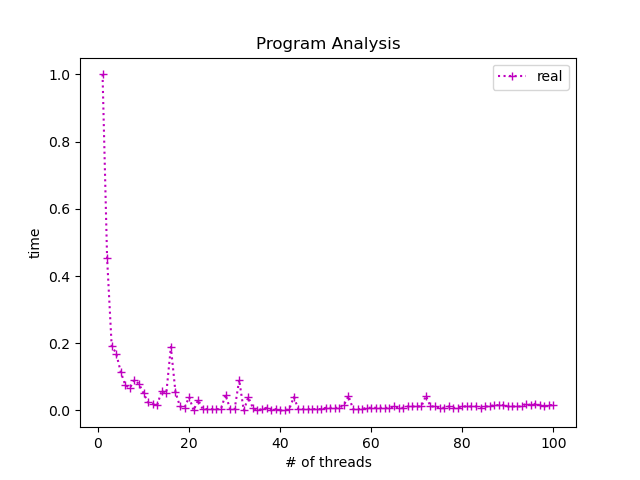
\includegraphics[height=0.3\textheight]{time.png}
      \caption{Execution Time}
    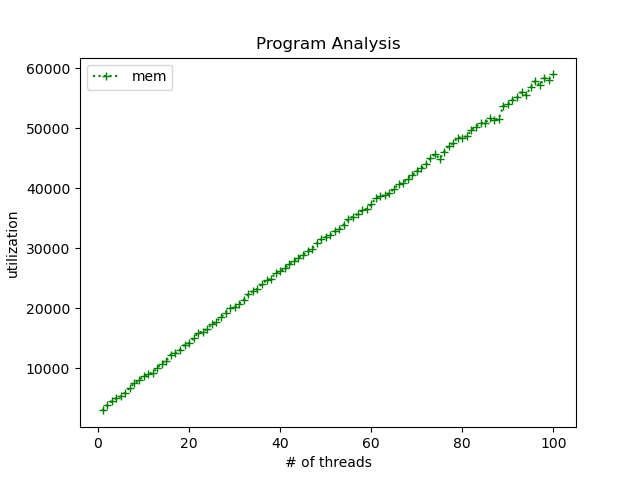
\includegraphics[height=0.3\textheight]{mem_util.png}
      \caption{Memory Utilization}
    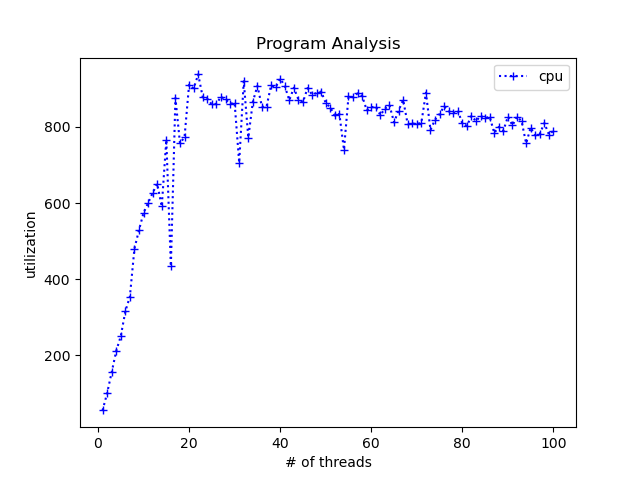
\includegraphics[height=0.3\textheight]{cpu_util.png}
    \caption{CPU Utilization}
  \end{figure}

  \clearpage
  \section*{Conclusion}
  Multiple threads allow multiple requests to be executed at the same time. This simple idea of concurrency improves
  program performances drastically, the figures above are drawn by testing on 200 images, with threads ranging from 1 to 100.
  
  As you can see in Figure 1, the real time it takes for this program to execute decreases as threads increases.
  It isn't a linear drop either, as a thread is introduced the runtime is cutdown by half. And as you introduce
  more threads the runtime decreases even more until it flattens out, indicating no more change. So, we can infer
  that after some x number of threads the effects on runtime are the same.

  Figure 2, there is a linear trend between memory utilization and the number of threads. This information isn't that shocking,
  since each thread has its own stack which requires some x bytes of memory, and as you increase the threads, each thread will
  require its own x bytes of memory. Thus, memory utilization increases as the number of threads increase.

  Figure 3, is an interesting one, it shows the relationship between CPU utilization and the number of threads. We came to a conclusion that the
  relationship depends on many factors. Something you might need to take in consideration, would be the type of work each thread is doing, since
  the CPU utilization depends on the type of computation. A simple computation won't be able to utilize the cpu in the same way computationly heavy
  threads might, and if there is parallelism then each thread is able to execute these computaton concurrently, thus increasing CPU utilization.
  Another thing to consider might be the underlying thread implementation, how each thread is waiting, this decreases CPU utilization since there
  isn't any CPU cycles being made, as compared to when a thread doesn't implement locks. The hardware architecture may also effect the relationship
  between CPU utilization and the number of threads. But, in this case, we can conclude that CPU utilization increases as the number of threads increases.

  By comparing, all the figures, we were able to conclude that having some threading is better than no threading, and some threading is also
  better than too much threading. There is a T number of threads you want to shoot for, because you want to optimize you program without using
  using too much resources. We noticed that 10 threads gives the same performance as 100 threads and everything between it. The only difference
  being the amount of resources used. So, if we can achieve the same results with 10 threads then that's what we should aim for. Another thing we
  wanted to mention was that each program has a different T number of threads that works best for it, 10 threads seemed like the best choice for 200
  image rotations. A program with a much heavier computation and number of tasks would have a different T that works best for it, which would be also
  be a high value.

\end{document}
